\section{Self-Adaptive Systems}


Self-adaptive systems have been accepted as a promising approach to tackle context change. Self-adaptivesses is an approach in which the system
\emph{"evaluates its own behavior and changes behavior when the evaluation indicates that it is not accomplishing what the software is intended to do, or when better functionality or performance is possible."}\cite{laddaga_self_1997}.

%kramer et al. dream

Self-adaptive software aims to adjust various artifacts or attributes in response to changes in the self and in the context of a software system\cite{salehie_self-adaptive_2009}.

A key concept in self-adaptive systems is the awareness of the system. It has two aspects\cite{salehie_self-adaptive_2009}:
\begin{itemize}
   \item \emph{self-awareness} means a system is aware of its own states and behaviors.
   \item \emph{context-awareness} means that the system is aware of its context,
\end{itemize}

% Schilit et al.\cite{klein_survey_2008} define \emph{context} as \say{the sufficiently exact characterization of the situations of a system by means of perceivable information that is relevant for the adaptation of the system}.

Schilit et al.\cite{klein_survey_2008} define \emph{context adaptation} as \say{a system’s capability of gathering information about the domain it shares an interface with, evaluating this information and changing its observable behavior according to the current situation}.

\begin{figure}[!htb]
 \centering
 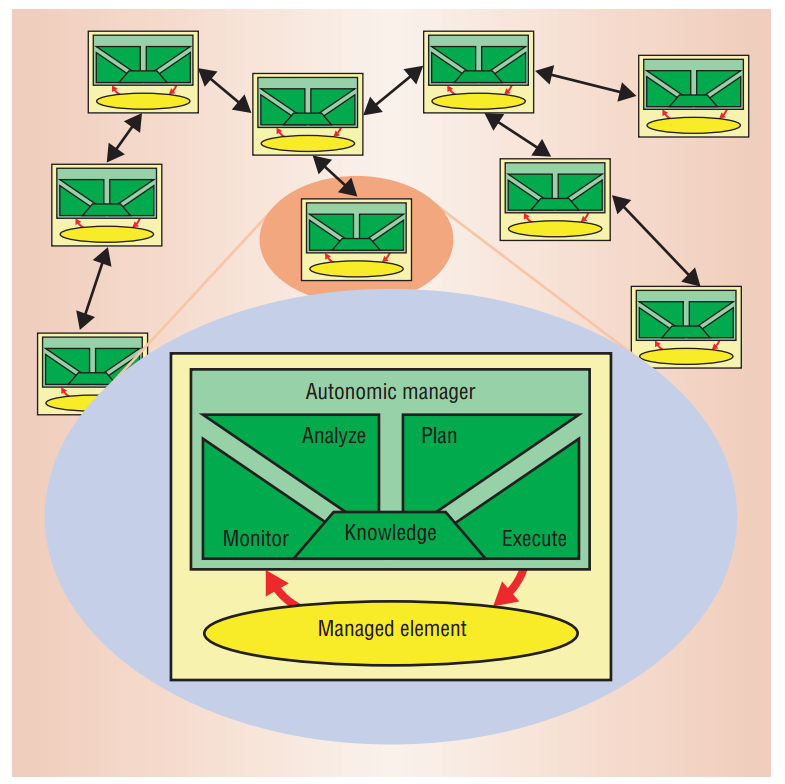
\includegraphics[width=\linewidth]{mape-k}
 \caption{CGM of the filling station advisor}
\label{fig:goal_model_filling_station_advisor}
\end{figure}

% laddaga1997: it should relies on software informed about its mission and about its construction and behavior.  This implies that the software has multiple ways of accomplishing its purpose, and has enough knowledge of its construction to make effective changes at runtime.

% Such software should include functionality for evaluating its behavior and performance, and the ability to replan and reconfigure its operations in order to improve its operation.  Self adaptive software should also include a set of components for each major function, along with descriptions of the components, so that components of systems can be selected and scheduled at runtime, in response to the evaluators.

% It also requires the ability to impedance match input/output of sequenced components, and the ability to generate some of this code from specifications. In addition, we seek this new basis of adaptation to be applied at runtime, as opposed to development/design-time, or as a maintenance activity.


% mape-k

% different approaches ref salehie

% challenges

%
% A self-managed software architecture is one in which components automatically configure their interaction in a way that is compatible with an overall architectural specification and achieves the goals of the system\cite{kramer_self-managed_2007}.

% Component Control
% include the capability to support component creation, deletion and interconnection.

% include facilities to report the current status of components to higher layers and also include the capability to support component creation, deletion and interconnection.
% adjust the operating parameters of components
% self-tuning algorithms, event and status reporting to higher levels and operations to support modification – component addition, deletion and interconnection.
% situation is met that the current configuration of components is not designed to deal with, this layer detects this failure and reports it to higher layers.



% Change Management

% Goal Management
